\documentclass[a4paper]{article}
\usepackage[margin=1.25in]{geometry}
\usepackage{bookmark}

\usepackage{amsmath}
\usepackage{amssymb}
\allowdisplaybreaks
\newcommand\numberthis{\addtocounter{equation}{1}\tag{\theequation}}

\usepackage{graphicx}
\usepackage{float}

\renewcommand{\baselinestretch}{1.15}
\setlength{\parindent}{0pt}

\usepackage{pdflscape}
\usepackage{xltabular}

\usepackage{multirow}
\usepackage{tabularx}
\newcolumntype{L}{>{\centering\arraybackslash}X}

\title{CS1.404: Assignment 1}
\author{Himanshu Singh}
\date{\today}

\begin{document}

\maketitle

\section{Trid Function}

$$f(\textbf{x}) = \sum_{i=1}^d (x_i - 1)^2 - \sum_{i=2}^d x_{i-1} x_i$$

\subsection{Jacobian and Hessian}

\begin{align*}
\nabla f(\textbf{x}) &=
    \begin{bmatrix}
        2 x_1 - x_2 - 2 \\
        2 x_2 - x_1 - x_3 - 2 \\
        2 x_3 - x_2 - x_4 - 2 \\
        \vdots \\
        2 x_{d-1} - x_{d-2} - x_d - 2 \\
        2 x_d - x_{d-1} - 2 \\
    \end{bmatrix}
\end{align*}

\begin{align*}
\nabla^2 f(\textbf{x}) &=
    \begin{bmatrix}
        2 & -1 & 0 & \dots & 0 \\
        -1 & 2 & -1 & \dots & 0 \\
        0 & -1 & 2 & \dots & 0 \\
        0 & 0 & -1 & \dots & 0 \\
        \vdots & \vdots & \vdots & \ddots & -1 \\
        0 & 0 & 0 & 0 & 2 \\
    \end{bmatrix}
\end{align*}

\subsection{Calculation of Minima}

We know from the SOSC for minima that $\textbf{x}^*$ is a local minima of the function $f(\textbf{x})$, if the following conditions hold.
\begin{align*}
&\nabla f(\textbf{x}^*) = \textbf{0} \\
&\implies{} 2 x_1 - x_2 = 2 \\ 
&\implies{} 2 x_{i} - x_{i-1} - x_{i+1} = 2 &&\forall i \in [2, d-1] \\
&\implies{} 2 x_d - x_{d-1} = 2 \numberthis \label{trid-sosc-1} \\ \\
&\textbf{y}^T \nabla^2 f(\textbf{x}^*) \textbf{y} > 0 &&\forall \textbf{y} \in \mathbb{R}^d \\
&\implies \begin{bmatrix} 2y_1 - y_2 & \dots & 2y_i - y_{i-1} - y_{i+1} & \dots & 2y_{d} - y_{d-1} \end{bmatrix} ^T \textbf{y} > 0 &&\forall \textbf{y} \in \mathbb{R}^d \\
&\implies 2 \left(\sum_{i=1}^d y_i^2 - \sum_{i=2}^d y_{i-1} y_i\right) > 0 &&\forall \textbf{y} \in \mathbb{R}^d \\
&\implies 2 \left(\sum_{i=1}^d y_i^2 - \sum_{i=2}^d y_{i-1} y_i\right) > 0 &&\forall \textbf{y} \in \mathbb{R}^d \\
&\implies \left(\sum_{i=2}^d y_{i-1}^2 + y_i^2 - 2y_{i-1} y_i\right) + y_1^2 + y_d^2 > 0 &&\forall \textbf{y} \in \mathbb{R}^d \\
&\implies \left(\sum_{i=2}^d (y_{i-1} - y_i)^2 \right) + y_1^2 + y_d^2 > 0 &&\forall \textbf{y} \in \mathbb{R}^d \numberthis \label{trid-sosc-2}
\end{align*}

Assuming $x_i = i(d + 1 - i)$, and substituting, we see that the inequalities \eqref{trid-sosc-1} hold; while the inequality \eqref{trid-sosc-2} holds regardless of $\textbf{x}$. Thus,
\begin{align*}
\textbf{x}^* = (d, 2d - 2, 3d - 6, \ldots{}, d) \numberthis \label{trid-minima}
\end{align*}

\subsection{Convergence of Algorithms}

For the given test case, all the algorithms converged to the local minima $\textbf{x}^* = (2, 2)$.

\subsection{Plots}

\begin{figure}[H]
      \centering
      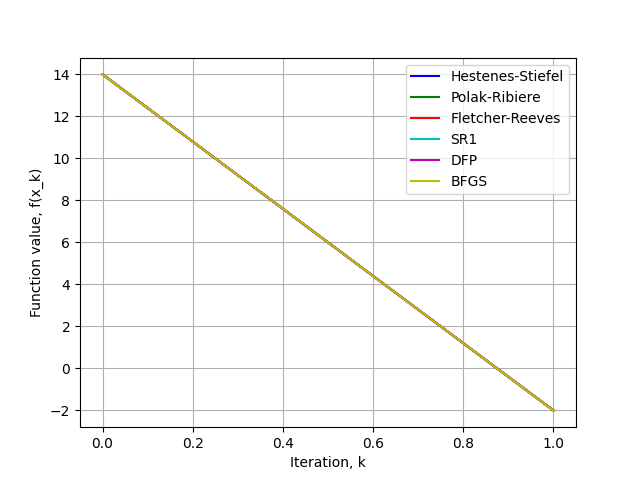
\includegraphics[width=.65\textwidth]{images/trid_function_vals.png}
      \caption{$f(\textbf{x}_k)$ vs $k$, for $\textbf{x}_0 = (-2, -2)$}
\end{figure}

\begin{figure}[H]
    \centering
    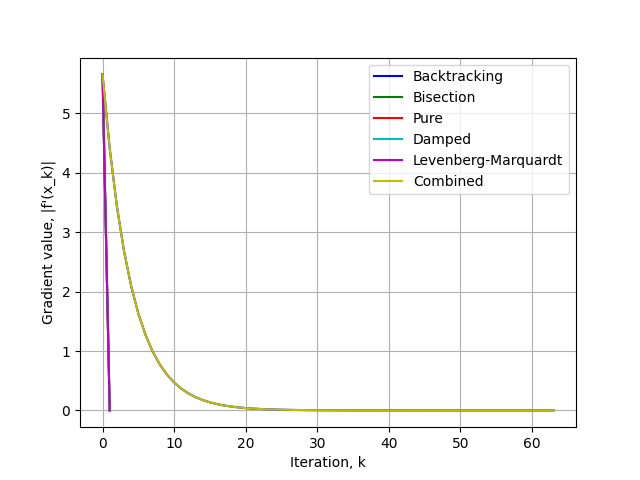
\includegraphics[width=.65\textwidth]{images/trid_function_grad.png}
    \caption{$|\nabla f(\textbf{x}_k)|$ vs $k$, for $\textbf{x}_0 = (-2, -2)$}
\end{figure}

\begin{figure}[H]
    \centering
    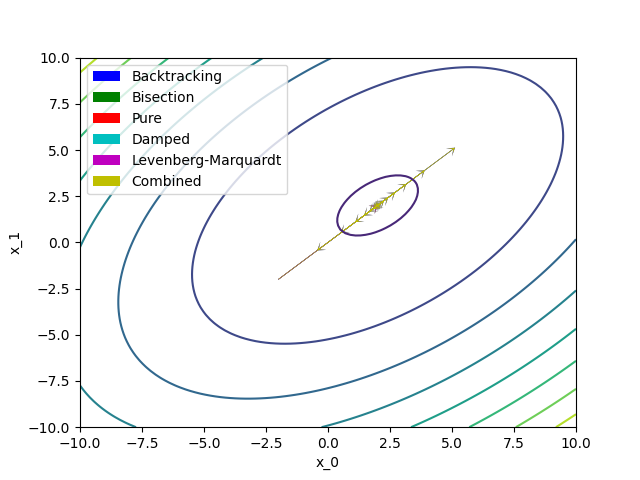
\includegraphics[width=.65\textwidth]{images/trid_function_cont.png}
    \caption{Contour plot, with direction of updates for $\textbf{x}_0 = (-2, -2)$}
\end{figure}

\section{Three Hump Camel}

$$f(\textbf{x}) = 2 x_1^2 - 1.05 x_1^4 + \frac{x_1^6}{6} + x_1 x_2 + x_2^2$$

\subsection{Jacobian and Hessian}

\begin{align*}
\nabla f(\textbf{x}) &=
    \begin{bmatrix}
        4 x_1 - 4.2 x_1^3 + x_1^5 + x_2 \\
        x_1 + 2 x_2
    \end{bmatrix}
\end{align*}

\begin{align*}
\nabla^2 f(\textbf{x}) &=
    \begin{bmatrix}
        5 x_1^4 - 12.6 x_1^2 + 4 & 1 \\
        1 & 2 \\
    \end{bmatrix}
\end{align*}

\subsection{Calculation of Minima}

We know from the SOSC for minima that $\textbf{x}^*$ is a local minima of the function $f(\textbf{x})$, if the following conditions hold.
\begin{align*}
&\nabla f(\textbf{x}^*) = \textbf{0} \\
&\implies 4 x_1 - 4.2 x_1^3 + x_1^5 + x_2 = 0 \numberthis \label{threehump-sosc-1} \\
&\phantom{\implies} \ \ x_1 + 2 x_2 = 0 \numberthis \label{threehump-sosc-2} \\ \\
&\textbf{y}^T \nabla^2 f(\textbf{x}^*) \textbf{y} > 0 &&\forall \textbf{y} \in \mathbb{R}^2 \\
&\implies y_1^2 (5 x_1^4 - 12.6 x_1^2 + 4) + 2 y_1 y_2 + 2 y_2^2 > 0 &&\forall y_1, y_2 \in \mathbb{R} \numberthis \label{threehump-sosc-3}
\end{align*}

Solving \eqref{threehump-sosc-1} and \eqref{threehump-sosc-2}, we get
\begin{align*}
    \left\{\textbf{x}^*\right\} = \left\{(-1.7476, 0.8738), (-1.0705, 0.5353), (0, 0), (1.0705, -0.5353), (1.7476, -0.8738)\right\} \numberthis \label{threehump-sosc-4}
\end{align*}

Checking satisfiability of inequality \eqref{threehump-sosc-3} for all possibilities \eqref{threehump-sosc-4}, we get
\begin{align*}
\left\{\textbf{x}^*\right\} = \left\{(-1.7476, 0.8738), (0, 0), (1.7476, -0.8738)\right\} \numberthis \label{threehump-minima}
\end{align*}

\subsection{Convergence of Algorithms}

For the given test cases, all the algorithms converged to one of the local minimas.

\subsection{Plots}

\begin{figure}[H]
      \centering
      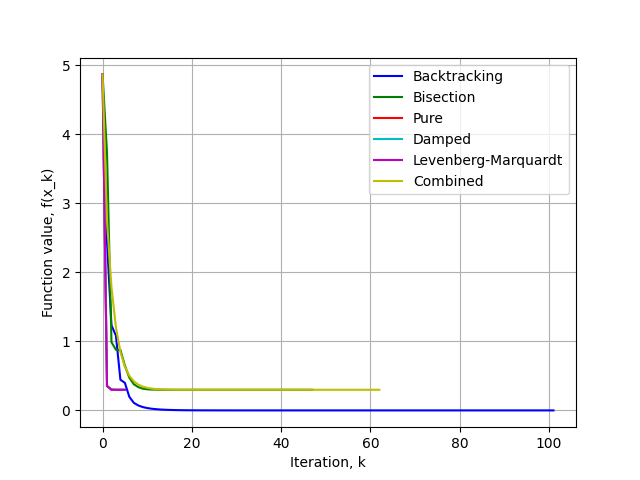
\includegraphics[width=.65\textwidth]{images/three_hump_camel_function_vals.png}
      \caption{$f(\textbf{x}_k)$ vs $k$, for $\textbf{x}_0 = (-2, -1)$}
\end{figure}

\begin{figure}[H]
    \centering
    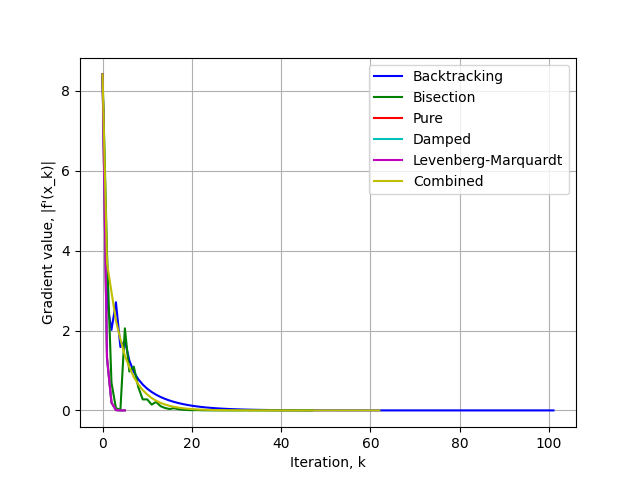
\includegraphics[width=.65\textwidth]{images/three_hump_camel_function_grad.png}
    \caption{$|\nabla f(\textbf{x}_k)|$ vs $k$, for $\textbf{x}_0 = (-2, -1)$}
\end{figure}

\begin{figure}[H]
    \centering
    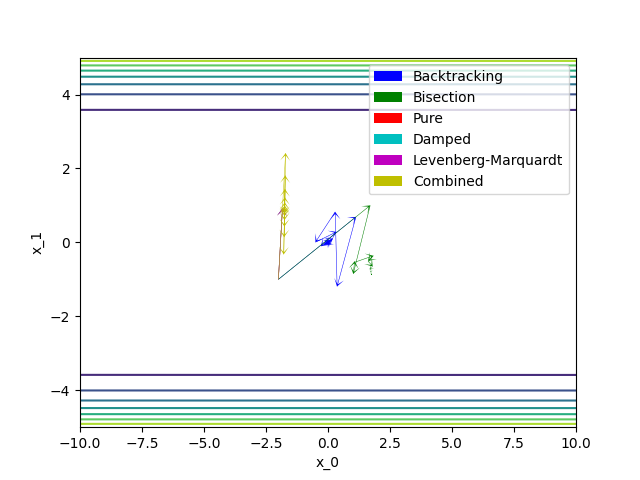
\includegraphics[width=.65\textwidth]{images/three_hump_camel_function_cont.png}
    \caption{Contour plot, with direction of updates for $\textbf{x}_0 = (-2, -1)$}
\end{figure}

\section{Styblinski-Tang Function}

$$f(\textbf{x}) = \frac{1}{2} \sum_{i=1}^d (x_i^4 - 16 x_i^2 + 5 x_i)$$

\subsection{Jacobian and Hessian}

\begin{align*}
\nabla f(\textbf{x}) &=
    \begin{bmatrix}
        2 x_1^3 - 16 x_1 + \cfrac{5}{2} \\
        2 x_2^3 - 16 x_2 + \cfrac{5}{2} \\
        \vdots \\
        2 x_d^3 - 16 x_d + \cfrac{5}{2} \\
    \end{bmatrix}
\end{align*}

\begin{align*}
\nabla^2 f(\textbf{x}) &=
    \begin{bmatrix}
        6 x_1^2 - 16 & 0 & \dots & 0 \\
        0 & 6 x_2^2 - 16 & \dots & 0 \\
        \vdots & \vdots & \ddots & 0 \\
        0 & 0 & 0 & 6 x_d^2 - 16 \\
    \end{bmatrix}
\end{align*}

\subsection{Calculation of Minima}

We know from the SOSC for minima that $\textbf{x}^*$ is a local minima of the function $f(\textbf{x})$, if the following conditions hold.
\begin{align*}
&\nabla f(\textbf{x}^*) = \textbf{0} \\
&\implies 2 x_i^3 - 16 x_i + \cfrac{5}{2} = 0 &&\forall i \in [1, d] \\
&\implies x_i \approx -2.9035, 0.15673, 2.7468 &&\forall i \in [1, d] \numberthis \label{sty-sosc-1} \\ \\
&\textbf{y}^T \nabla^2 f(\textbf{x}^*) \textbf{y} > 0 &&\forall \textbf{y} \in \mathbb{R}^d \\
&\implies y_i^2 (6 x_i^2 - 16) > 0 &&\forall y_i \in \mathbb{R}, i \in [1, d] \\
&\implies x_i^2 > \cfrac{8}{3} &&\forall i \in [1, d] \\
&\implies |x_i| > 1.63 &&\forall i \in [1, d] \numberthis \label{sty-sosc-2}
\end{align*}

Combining \eqref{sty-sosc-1} and \eqref{sty-sosc-2}, we get $x_i = -2.9035, 2.7468$. Thus, the set of local minimas is
\begin{align*}
\left\{\textbf{x}^*\right\} = \left\{-2.9035, 2.7468\right\}^d \numberthis \label{sty-minima}
\end{align*}

\subsection{Convergence of Algorithms}

\begin{enumerate}

\item Pure and Damped Newton's Method converged, for all except the first test case. Notably, the Pure Netwon's Method returned $\textbf{x} = (0.157, 0.157, 0.157, 0.157)$ on failure, which as we saw earlier satisfies the FONC.

\item Steepest Descent with Backtracking, Steepest Descent with Bisection search, Levenberg-Marquardt Modification and Combined Damped Netwon's Method converged to one of the local minimas, for all the test cases.

\end{enumerate}

\subsection{Plots}

\begin{figure}[H]
      \centering
      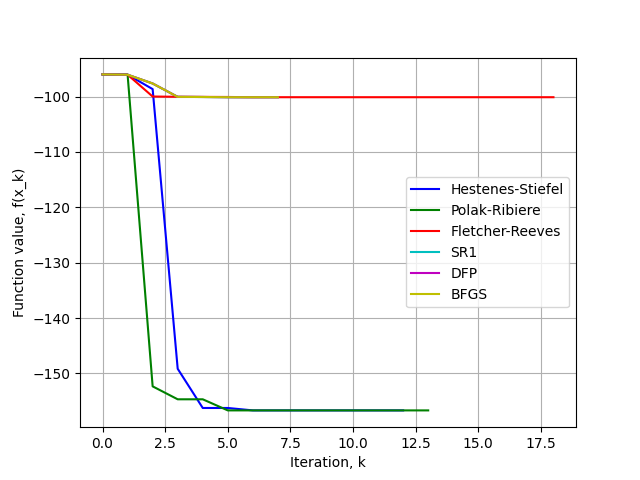
\includegraphics[width=.65\textwidth]{images/styblinski_tang_function_vals.png}
      \caption{$f(\textbf{x}_k)$ vs $k$, for $\textbf{x}_0 = (3, 3, 3, 3)$}
\end{figure}

\begin{figure}[H]
    \centering
    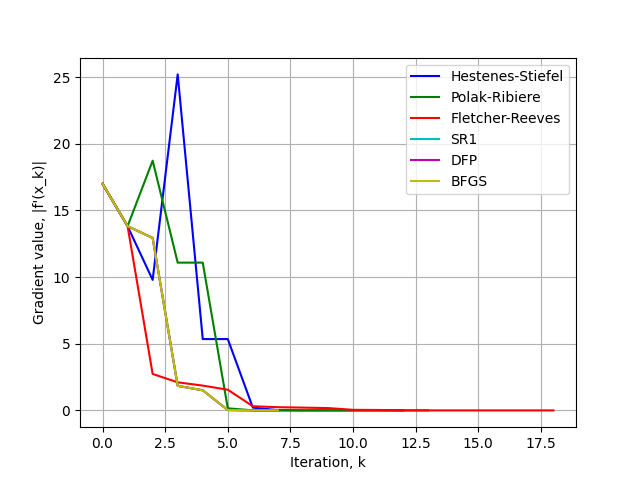
\includegraphics[width=.65\textwidth]{images/styblinski_tang_function_grad.png}
    \caption{$|\nabla f(\textbf{x}_k)|$ vs $k$, for $\textbf{x}_0 = (3, 3, 3, 3)$}
\end{figure}

\section{Rosenbrock Function}

$$f(\textbf{x}) = \sum_{i=1}^{d-1} [ 100(x_{i+1} - x_i^2)^2 + (x_i - 1)^2 ]$$

\subsection{Jacobian and Hessian}

\begin{align*}
\nabla f(\textbf{x}) &=
    \begin{bmatrix}
        400 x_1 (x_1^2 - x_2) + 2 (x_1 - 1) \\
        400 x_2 (x_2^2 - x_3) + 2 (x_2 - 1) + 200 (x_2 - x_1^2) \\
        400 x_3 (x_3^2 - x_4) + 2 (x_3 - 1) + 200 (x_3 - x_2^2) \\
        \vdots \\
        400 x_{d-1} (x_{d-1}^2 - x_k) + 2 (x_{d-1} - 1) + 200 (x_{d-1} - x_{d-2}^2) \\
        200 (x_d - x_{d-1}^2) \\
    \end{bmatrix}
\end{align*}

\begin{align*}
\nabla^2 f(\textbf{x}) &=
    \begin{bmatrix}
        1200 x_1^2 - 400 x_2 + 2 & -400 x_1 & 0 & \dots & 0 \\
        -400 x_1 & 1200 x_2^2 - 400 x_3 + 202 & -400 x_2 & \dots & 0 \\
        0 & -400 x_2 & 1200 x_3^2 - 400 x_4 + 202 & \dots & 0 \\
        0 & 0 & -400 x_3 & \dots & 0 \\
        \vdots & \vdots & \vdots & \ddots & -400 x_{d-1} \\
        0 & 0 & 0 & -400 x_{d-1} & 200 \\
    \end{bmatrix}
\end{align*}

\subsection{Convergence of Algorithms}

\begin{enumerate}

\item Pure Newton's Method, Damped Newton's Method, Levenberg-Marquardt Modification and Combined Damped Netwon's Method converged, for all except the third test case.

\item Steepest Descent with Backtracking and Bisection search converged for all the test cases.

\end{enumerate}

\subsection{Plots}

\begin{figure}[H]
      \centering
      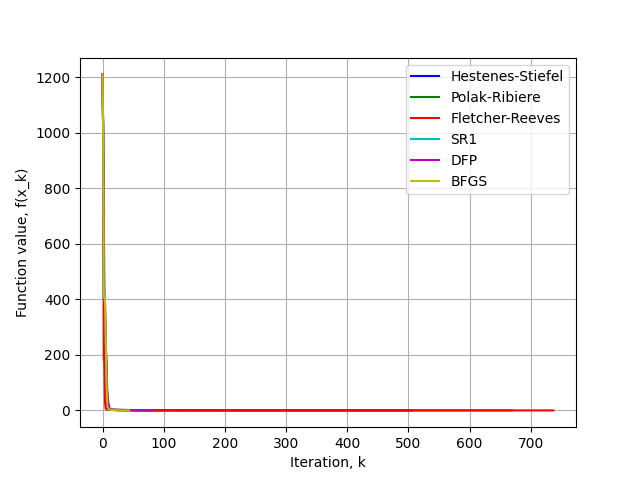
\includegraphics[width=.65\textwidth]{images/rosenbrock_function_vals.png}
      \caption{$f(\textbf{x}_k)$ vs $k$, for $\textbf{x}_0 = (-2, 2, 2, 2)$}
\end{figure}

\begin{figure}[H]
    \centering
    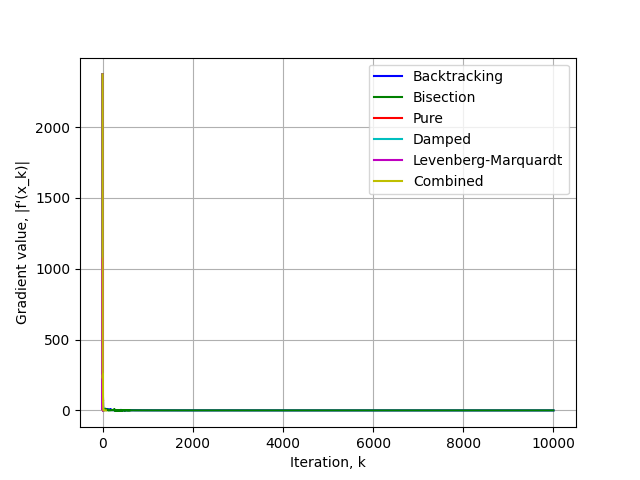
\includegraphics[width=.65\textwidth]{images/rosenbrock_function_grad.png}
    \caption{$|\nabla f(\textbf{x}_k)|$ vs $k$, for $\textbf{x}_0 = (-2, 2, 2, 2)$}
\end{figure}

\section{Root of Square Function}

$$f(\textbf{x}) = \sqrt{1 + x_1^2} + \sqrt{1 + x_2^2}$$

\subsection{Jacobian and Hessian}

\begin{align*}
\nabla f(\textbf{x}) &=
    \begin{bmatrix}
        \cfrac{x_1}{\sqrt{1 + x_1^2}} \\
        \cfrac{x_2}{\sqrt{1 + x_2^2}}
    \end{bmatrix}
\end{align*}

\begin{align*}
\nabla^2 f(\textbf{x}) &=
    \begin{bmatrix}
        \cfrac{1}{\sqrt{(1 + x_1^2)^3}} & 0 \\
        0 & \cfrac{1}{\sqrt{(1 + x_1^2)^3}} \\
    \end{bmatrix}
\end{align*}

\subsection{Calculation of Minima}

We know from the SOSC for minima that $\textbf{x}^*$ is a local minima of the function $f(\textbf{x})$, if the following conditions hold.
\begin{align*}
&\nabla f(\textbf{x}^*) = \textbf{0} \\
&\implies \cfrac{x_i}{\sqrt{1 + x_i^2}} = 0 &&\forall i \in [1, 2] \\
&\implies x_i = 0 &&\forall i \in [1, 2] \numberthis \label{rootsq-sosc-1} \\ \\
&\textbf{y}^T \nabla^2 f(\textbf{x}^*) \textbf{y} > 0 &&\forall \textbf{y} \in \mathbb{R}^2 \\
&\implies \cfrac{y_i^2}{\sqrt{(1 + x_i^2)^3}} > 0 &&\forall y_i \in \mathbb{R}, i \in [1, 2] \\
&\implies (1 + x_i^2)^3 > 0 &&\forall i \in [1, 2] \\
&\implies x_i^2 > -1 &&\forall i \in [1, 2] \numberthis \label{rootsq-sosc-2}
\end{align*}

Since \eqref{rootsq-sosc-2} always hold, from \eqref{rootsq-sosc-1} we get $x_i = 0$. Thus, the local minima is
\begin{align*}
\textbf{x}^* = (0, 0) \numberthis \label{rootsq-minima}
\end{align*}

\subsection{Convergence of Algorithms}

\begin{enumerate}

\item Pure Newton's Method and Levenberg-Marquardt Modification converged, only for the second test case.

\item Steepest Descent with Backtracking, Steepest Descent with Bisection search, Damped Newton's Method and Combined Damped Netwon's Method converged to the local minima $\textbf{x}^* = (0, 0)$, for all the test cases.

\end{enumerate}

\subsection{Plots}

\begin{figure}[H]
      \centering
      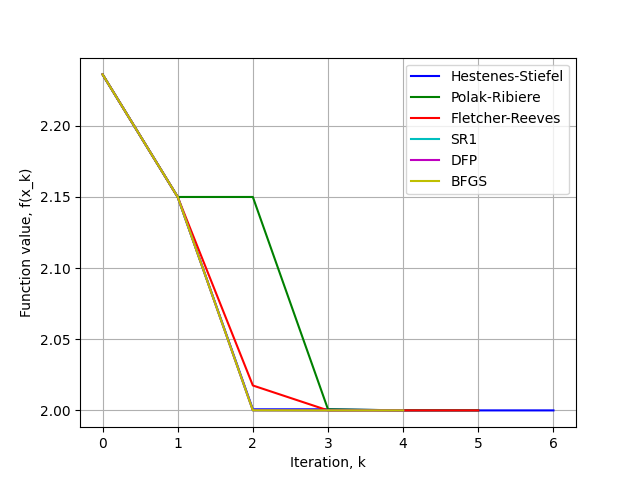
\includegraphics[width=.65\textwidth]{images/func_1_vals.png}
      \caption{$f(\textbf{x}_k)$ vs $k$, for $\textbf{x}_0 = (-0.5, 0.5)$}
\end{figure}

\begin{figure}[H]
    \centering
    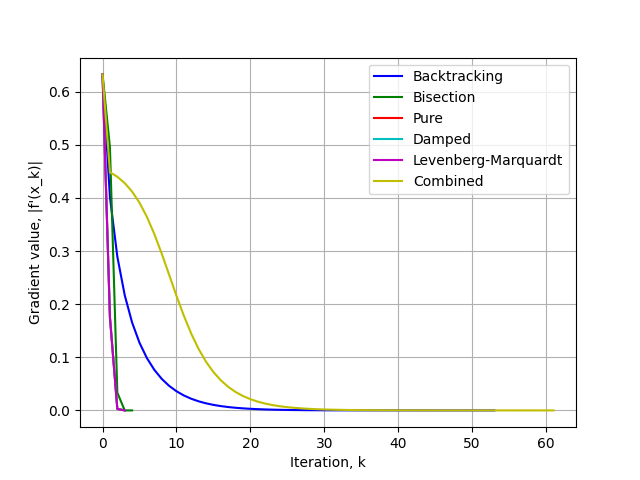
\includegraphics[width=.65\textwidth]{images/func_1_grad.png}
    \caption{$|\nabla f(\textbf{x}_k)|$ vs $k$, for $\textbf{x}_0 = (-0.5, 0.5)$}
\end{figure}

\begin{figure}[H]
    \centering
    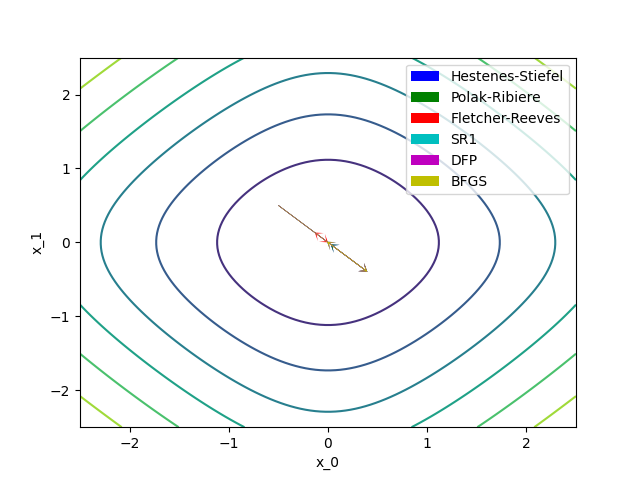
\includegraphics[width=.65\textwidth]{images/func_1_cont.png}
    \caption{Contour plot, with direction of updates for $\textbf{x}_0 = (-0.5, 0.5)$}
\end{figure}

\begin{landscape}
    \section*{Appendix: Output for all test cases}
    \begin{xltabular}{\linewidth}{cLLLLLLLL}
        \hline
        Test Case & Function & Initial Point & Backtracking & Bisection & Pure & Damped & Levenberg-Marquardt & Combined \\
        \hline
        \endhead
        1 & Trid & (-2, -2) & (2, 2) & (2, 2) & (2, 2) & (2, 2) & (2, 2) & (2, 2) \\
        \hline
        2 & \multirow{4}{*}{Three Hump Camel} & (-2, 1) & (-1.748, 0.874) & (-1.748, 0.874) & (-1.748, 0.874) & (-1.748, 0.874) & (-1.748, 0.874) & (0, 0) \\
        3 & & (2, -1) & (1.748, -0.874) & (1.748, -0.874) & (1.748, -0.874) & (1.748, -0.874) & (1.748, -0.874) & (0, 0) \\
        4 & & (-2, -1) & (0, 0) & (1.748, -0.874) & (-1.748, 0.874) & (-1.748, 0.874) & (-1.748, 0.874) & (-1.748, 0.874) \\
        5 & & (2, 1) & (0, 0) & (-1.748, 0.874) & (1.748, -0.874) & (1.748, -0.874) & (1.748, -0.874) & (1.748, -0.874) \\
        \hline
        6 & \multirow{4}{*}{Rosenbrock} & (2, 2, 2, -2) & (1, 1, 1, 1) & (1, 1, 1, 1) & (1, 1, 1, 1) & (1, 1, 1, 1) & (1, 1, 1, 1) & (1, 1, 1, 1) \\
        7 & & (2, -2, -2, 2) & (1, 1, 1, 1) & (1, 1, 1, 1) & (1, 1, 1, 1) & (1, 1, 1, 1) & (1, 1, 1, 1) & (1, 1, 1, 1) \\
        8 & & (-2, 2, 2, 2) & (1, 1, 1, 1) & (1, 1, 1, 1) & (-0.776, 0.613, 0.382, 0.146) & (-0.776, 0.613, 0.382, 0.146) & (-0.776, 0.613, 0.382, 0.146) & (-0.776, 0.613, 0.382, 0.146) \\
        9 & & (3, 3, 3, 3) & (1, 1, 1, 1) & (1, 1, 1, 1) & (1, 1, 1, 1) & (1, 1, 1, 1) & (1, 1, 1, 1) & (1, 1, 1, 1) \\
        \hline
        10 & \multirow{4}{*}{Styblinski-Tang} & (0, 0, 0, 0) & (-2.904, -2.904, -2.904, -2.904) & (-2.904, -2.904, -2.904, -2.904) & (0.157, 0.157, 0.157, 0.157) & (0, 0, 0, 0) & (-2.904, -2.904, -2.904, -2.904) & (-2.904, -2.904, -2.904, -2.904) \\
        11 & & (3, 3, 3, 3) & (-2.904, -2.904, -2.904, -2.904) & (-2.904, -2.904, -2.904, -2.904) & (2.747, 2.747, 2.747, 2.747) & (2.747, 2.747, 2.747, 2.747) & (2.747, 2.747, 2.747, 2.747) & (2.747, 2.747, 2.747, 2.747) \\
        12 & & (-3, -3, -3, -3) & (-2.904, -2.904, -2.904, -2.904) & (-2.904, -2.904, -2.904, -2.904) & (-2.904, -2.904, -2.904, -2.904) & (-2.904, -2.904, -2.904, -2.904) & (-2.904, -2.904, -2.904, -2.904) & (-2.904, -2.904, -2.904, -2.904) \\
        13 & & (3, -3, 3, -3) & (2.747, -2.904, 2.747, -2.904) & (2.747, -2.904, 2.747, -2.904) & (2.747, -2.904, 2.747, -2.904) & (2.747, -2.904, 2.747, -2.904) & (2.747, -2.904, 2.747, -2.904) & (2.747, -2.904, 2.747, -2.904) \\
        \hline
        14 & \multirow{3}{*}{Root Square} & (3, 3) & (0, 0) & (0, 0) & (-8.72e+115, -8.72e+115) & (0, 0) & (-8.72e+115, -8.72+115) & (0, 0) \\
        15 & & (-0.5, 0.5) & (0, 0) & (0, 0) & (0, 0) & (0, 0) & (0, 0) & (0, 0) \\
        16 & & (-3.5, 0.5) & (0, 0) & (0, 0) & (4.9e+14, 0) & (0, 0) & (4.9e+14, 0) & (0, 0) \\
        \hline
    \end{xltabular}
\end{landscape}

\end{document}
